According to \citep{Hothorn.2006} an algorithm for recursive partitionig is called unbiased when, under the conditions of the null hypothesis of independence between a response $y$ an feature $\textbf{x}_{1},...\textbf{x}_{p}$ the probability of selecting feature $\textbf{x}_{1}$ is $1/p$ for all $j = 1,...,p$ regardless of the measurement scales or number of missing values. 

This definition may be surprising at first, since if there is no dependency between the target and the features, one would not want to perform a split anyway and would try to prevent this through appropriate pruning procedures.
However, the idea behind this is that if, in the case of independence, a feature with, for example, a large number of possible splitpoints is selected more frequently as a splitting variable than a feature with a smaller number of splitpoints, the former could also be incorrectly selected more frequently as a splitting variable if there is a dependency on the response for the second feature.
\citep{Loh.2014}


In the discussion on the Paper Fifty Years of Classification and Regression Trees of \citep{Loh.2014}, Carolin Strobl's statement on selection bias is therefore very clear:


{\par\centering \textit{"One should think that the results shown here, and in many previous studies that Wei-Yin Loh has summarized in his paper, are so clear that any statistically educated person should never
want to use a biased recursive partitioning algorithm again."}\par}

So if SLIM is the only unbiased algorithm, it would have to be discarded immediately according to this statement. However, this will be investigated in detail in the following.



\subsection{Simulation selection bias independence}
In order to empirically investigate whether the four algorithms presented actually correspond to the respective groups (biased and unbiased) using the definition of \citep{Hothorn.2006}, two different simulation were carried out.

In the first scenario only numerical features are used, whereas in the second scenario numerical features and additionally one binary and two categorical features are considered.

\paragraph{Independence numeric}
\begin{itemize}
    \item $\textbf{x}_{1}, \textbf{x}_{2} \sim U(0,1)$
    \item $\textbf{x}_3$ uniformly distributed on the set $\{0, 0.1,..., 0.9, 1\}$
    \item $\textbf{x}_4$ uniformly distributed on the set $\{0, 0.01,..., 0.99, 1\}$
    \item $y \sim N(0,1)$
    \item sample size $n = 1000$
    \item 1000 simulation runs
\end{itemize}

The resulting frequencies are shown in Figure \ref{fig:selection_bias_independence_numeric} and are consistent with the expectations. SLIM actually prefers to select features with a higher number of splitpoints and therefore is biased. The other three methods select all four features about the same number of times.

\begin{figure}[!htb]
    \centering
    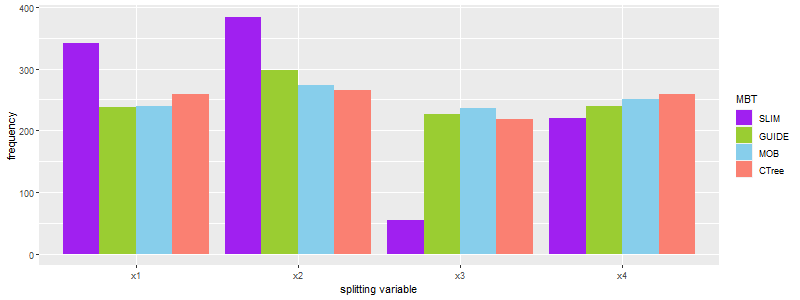
\includegraphics[width=16cm]{Figures/simulations/batchtools/selection_bias_general_10_01/independence_small.png}
    \caption{Simulated frequencies of selected splitting features for scenario independence numeric}
    \label{fig:selection_bias_independence_numeric}
\end{figure}

For the simulations in this chapter, each unique value was seen as a potential split point for SLIM.
However, as a possible correction approach for the selection bias in SLIM, I investigated how the number of quantiles considered as potential split points affects the selection bias and the performance (mean square error) of SLIM. The simulation setup and results are shown in the appendix. In summary, the selection bias can indeed be reduced by a smaller number of quantiles, but performance also suffers. In principle, it would be possible to consider the number of quantiles as a tuning parameter and to try to achieve the best possible trade off between selection bias and performance. 



\paragraph{Selection bias independence mixed}
\begin{itemize}
    \item $\textbf{x}_{1}, \textbf{x}_{2} \sim U(0,1)$ 
    \item $\textbf{x}_3$ uniformly distributed on the set $\{0, 0.1,..., 0.9, 1\}$ 
    \item $\textbf{x}_4  \sim Bern(0.5)$ 
    \item $\textbf{x}_5$ uniformly distributed on 5 factor levels (15 possible split sets) 
    \item $\textbf{x}_5$ uniformly distributed on 8 factor levels (128 possible split sets) %stirling number of second kind    
    \item $y \sim N(0,1)$
    \item sample size $n = 1000$
    \item 1000 simulation runs
\end{itemize}

The addition of categorical features in this scenario results in a different picture for the frequencies, as shown in Figure \ref{fig:selection_bias_independence_mixed}. Although the numerical variables are chosen with approximately equal frequency in the so-called "unbiased" methods, there are large deviations in the binary and categorical variables, which calls the designation "unbiased" into question.

\begin{figure}[!htb]
    \centering
    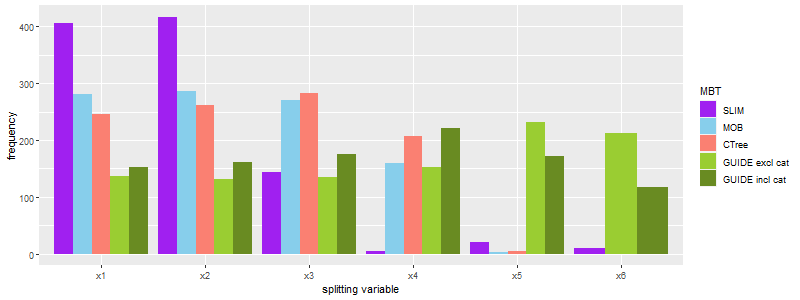
\includegraphics[width=16cm]{Figures/simulations/batchtools/selection_bias_general_10_01/independence.png}
    \caption{Simulated frequencies of selected splitting features for scenario independence mixed}
    \label{fig:selection_bias_independence_mixed}
\end{figure}










% Seite 6664


\vspace{1cm}




%\textbf{Test for selection bias:} $\chi^2$ goodness of fit test\\
%H0: the probabilities of the population are all equal (or are equal to an assumed probability distribution p)





